\documentclass[12pt,a4paper]{article}
\usepackage[utf8]{inputenc}
\usepackage[T1]{fontenc}
\usepackage[french]{babel}
\usepackage{graphicx}
\usepackage{amsmath}
\usepackage{listings}
\usepackage{xcolor}
\usepackage{hyperref}
\usepackage{enumitem}
\usepackage{geometry}
\usepackage{fancyhdr}

\geometry{a4paper, margin=2.5cm}

% Fix the header height
\setlength{\headheight}{16.35004pt}
\addtolength{\topmargin}{-0.996pt}

\pagestyle{fancy}
\fancyhf{}
\fancyhead[L]{
\includegraphics[height=12pt]{n7.png}}
\fancyhead[C]{Équipe KL-4}
\fancyhead[R]{\thepage}
\fancyfoot[C]{Simulateur d'Avion - 2025}

% Configuration des listings pour Java
\definecolor{javared}{rgb}{0.6,0,0}
\definecolor{javagreen}{rgb}{0.25,0.5,0.35}
\definecolor{javapurple}{rgb}{0.5,0,0.35}
\definecolor{javacomment}{rgb}{0.5,0.5,0.5}

\lstset{
    language=Java,
    basicstyle=\ttfamily\small,
    keywordstyle=\color{javapurple}\bfseries,
    stringstyle=\color{javared},
    commentstyle=\color{javacomment},
    numbers=left,
    numberstyle=\tiny\color{javacomment},
    stepnumber=1,
    numbersep=8pt,
    showspaces=false,
    showstringspaces=false,
    breaklines=true,
    frameround=ftff,
    frame=lines,
    backgroundcolor=\color{white},
    captionpos=b
}

\title{
    
\includegraphics[width=0.4\textwidth]{n7.png}\\[1cm]
    \textbf{Rapport Global - Projet Simulateur d'Avion}
}
\author{ASSKNID Walid - Équipe KL-4}
\date{\today}

\begin{document}

\maketitle
\thispagestyle{empty}

\tableofcontents
\newpage

\section{État d'avancement du projet}

\subsection{Progression globale}
À ce stade du projet, nous avons réalisé environ 30\% des fonctionnalités prévues. Cette première phase s'est concentrée sur la mise en place de l'architecture de base et l'implémentation des fonctionnalités essentielles.

\subsection{Fonctionnalités implémentées}
\begin{itemize}
    \item \textbf{Interface utilisateur de base} (80\%)
    \begin{itemize}
        \item Menu principal avec animations
        \item Système de navigation entre les écrans
        \item Boutons interactifs avec effets visuels
    \end{itemize}
    
    \item \textbf{Simulation de base} (40\%)
    \begin{itemize}
        \item Affichage des avions
        \item Contrôles basiques de vol
        \item Gestion des collisions (version initiale)
    \end{itemize}
    
    \item \textbf{Gestion des événements} (30\%)
    \begin{itemize}
        \item Interactions clavier/souris
        \item Sélection des avions
        \item Mise à jour en temps réel
    \end{itemize}
\end{itemize}

\section{Technologies Java utilisées}

\subsection{Bibliothèques principales}
\begin{itemize}
    \item \textbf{Java Swing}
    \begin{itemize}
        \item JFrame pour la fenêtre principale
        \item JPanel pour les différents écrans
        \item JButton pour les contrôles
        \item Timer pour les animations
    \end{itemize}
    
    \item \textbf{Java AWT}
    \begin{itemize}
        \item Graphics2D pour le rendu
        \item Image et ImageIO pour la gestion des images
        \item Event handling (MouseListener, KeyListener)
        \item Geometric shapes (Rectangle, Point)
    \end{itemize}
\end{itemize}

\subsection{Concepts de programmation}
\begin{itemize}
    \item \textbf{Programmation orientée objet}
    \begin{itemize}
        \item Héritage et polymorphisme
        \item Encapsulation
        \item Interfaces et classes abstraites
    \end{itemize}
    
    \item \textbf{Collections}
    \begin{itemize}
        \item List pour gérer les avions
        \item ArrayList pour les structures de données dynamiques
    \end{itemize}
    
    \item \textbf{Event-driven programming}
    \begin{itemize}
        \item Listeners pour les événements
        \item Callbacks et délégation
    \end{itemize}
\end{itemize}

\section{Architecture du projet}

\subsection{Diagramme de classes UML}
La figure suivante présente l'architecture globale du projet sous forme de diagramme UML :

\begin{figure}[!h]
    \centering
    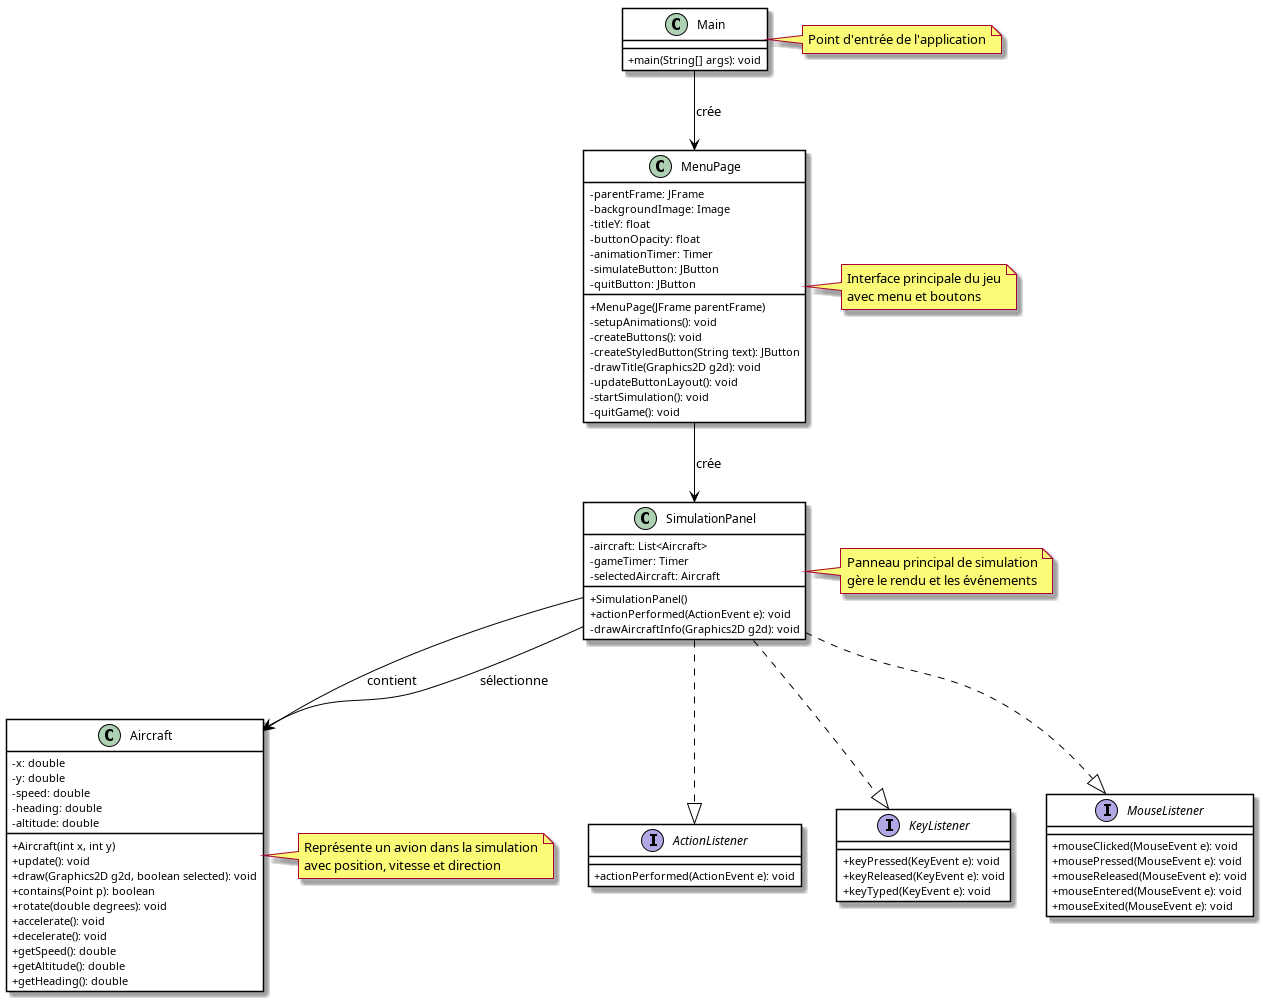
\includegraphics[width=1.0\textwidth]{Simulateur d'Avion.png}
    \caption{Diagramme de classes UML du simulateur d'avion}
\end{figure}

\subsection{Description des composants principaux}
\begin{itemize}
    \item \textbf{Main} : Point d'entrée de l'application, initialise la fenêtre principale
    \item \textbf{MenuPage} : Gère l'interface du menu principal avec animations
    \item \textbf{SimulationPanel} : Cœur de la simulation, gère le rendu et les interactions
    \item \textbf{Aircraft} : Représente un avion avec ses propriétés et comportements
\end{itemize}

% Ancienne version commentée
%\subsection{Diagramme de classes UML}
%La figure suivante présente l'architecture globale du projet sous forme de diagramme UML :
%
%\begin{figure}[!h]
%    \centering
%    \includegraphics[width=0.9\textwidth]{simulateur_avion_uml.png}
%    \caption{Diagramme de classes UML du simulateur d'avion}
%\end{figure}

\section{Prochaines étapes}

\subsection{Fonctionnalités à implémenter}
\begin{itemize}
    \item Système météorologique complet
    \item Gestion avancée du trafic aérien
    \item Planification de vol
    \item Interface utilisateur améliorée
    \item Système de missions
\end{itemize}

\subsection{Améliorations techniques}
\begin{itemize}
    \item Optimisation des performances
    \item Refactoring du code
    \item Tests unitaires
    \item Documentation complète
\end{itemize}

\section{Conclusion}
Cette première phase du projet a permis de mettre en place les fondations essentielles du simulateur. Bien que seulement 30\% du travail soit réalisé, les composants de base sont fonctionnels et l'architecture est extensible pour accueillir les futures fonctionnalités. Les prochaines itérations se concentreront sur l'ajout de fonctionnalités avancées et l'amélioration de l'expérience utilisateur.

\end{document} 